\documentclass[letter, 11pt]{article}
%% ================================
%% Packages =======================
\usepackage[utf8]{inputenc}      %%
\usepackage[T1]{fontenc}         %%
\usepackage{lmodern}             %%
\usepackage[spanish]{babel}      %%
\decimalpoint                    %%
\usepackage{fullpage}            %%
\usepackage{fancyhdr}            %%
\usepackage{graphicx}            %%
\usepackage{amsmath}             %%
\usepackage{amssymb}             %%
\usepackage{color}               %%
\usepackage{mdframed}            %%
\usepackage[colorlinks]{hyperref}%%
\usepackage{float}               %%
\usepackage{python}              %%
\usepackage[margin=1cm]{caption} %%
%% ================================
%% ================================

%% ================================
%% Page size/borders config =======
\setlength{\oddsidemargin}{0in}  %%
\setlength{\evensidemargin}{0in} %%
\setlength{\marginparwidth}{0in} %%
\setlength{\marginparsep}{0in}   %%
\setlength{\voffset}{-0.5in}     %%
\setlength{\hoffset}{0in}        %%
\setlength{\topmargin}{0in}      %%
\setlength{\headheight}{54pt}    %%
\setlength{\headsep}{1em}        %%
\setlength{\textheight}{8.5in}   %%
\setlength{\footskip}{0.5in}     %%
%% ================================
%% ================================

%% =============================================================
%% Headers setup, environments, colors, etc.
%%
%% Header ------------------------------------------------------
\fancypagestyle{firstpage}
{
  \fancyhf{}
  \lhead{
\includegraphics[height=4.5em]{LogoDFI.jpg}}
  \rhead{FI3104-1 \semestre\\
         Métodos Numéricos para la Ciencia e Ingeniería}
  \fancyfoot[C]{\thepage}
}

\pagestyle{plain}
\fancyhf{}
\fancyfoot[C]{\thepage}
%% -------------------------------------------------------------
%% Environments -------------------------------------------------
\newmdenv[
  linecolor=gray,
  fontcolor=gray,
  linewidth=0.2em,
  topline=false,
  bottomline=false,
  rightline=false,
  skipabove=\topsep
  skipbelow=\topsep,
]{ayuda}
%% -------------------------------------------------------------
%% Colors ------------------------------------------------------
\definecolor{gray}{rgb}{0.5, 0.5, 0.5}
%% -------------------------------------------------------------
%% Aliases ------------------------------------------------------
\newcommand{\scipy}{\texttt{scipy}}
%% -------------------------------------------------------------
%% =============================================================

%% =============================================================================
%% CONFIGURACION DEL DOCUMENTO =================================================
%% Llenar con la información pertinente al curso y la tarea
%%
\newcommand{\fechaentrega}{14/08/2019 23:59 hrs}
\newcommand{\semestre}{2019B}
%% =============================================================================
%% =============================================================================


\begin{document}
\thispagestyle{firstpage}

\begin{center}
  {\uppercase{\LARGE \bf Informe Tarea 3}}
\end{center}

\noindent{\Large Tomás Rojas C.}\\
\noindent{\Large RUT:19.688.339-8}\\
\noindent{\Large Github: @tomasrojasc}


%% =============================================================================
%% =============================================================================
\section{Introducción.}

El objetivo de esta tarea es permitir mejor conocimiento
de los métodos de interpolación, sus ventajas, y
desventajas. En particular, en este informe se compararán
las interpolaciones con polinomios versus las
interpolaciones spline.

\subsection{Sobre los gráficos extra.}

En este informe hay gráficos que no fueron pedidos pero que es interesante ver, los códigos para generarlos se pueden encontrar en ``p1\_cosas\_al\_margen.py'' para la parte de la pregunta 1.


\section{Problema 1.}

En este primer ejercicio, vamos a utilizar los métodos de interpolación antes mencionados para ver cómo se desempeñan al interpolar la función:

\begin{equation}
  f(x)=e^{-\frac{x^2}{0.05}}
\end{equation}

\subsection{Interpolación con método de Lagrange.}

Partimos con un arreglo de 5 datos equiespaciados, esto nos da
como resultado la figura \ref{P1_1}. Es facil notar que la
interpolación, marcada por la línea continua naranja, no se
acerca mucho a lo esperado, marcado por línea segmentada verde,
de hecho solo comparte los puntos que se usaron para la
interpolación, que es al mismo tiempo la cantidad mínima de
puntos que se pueden tener bien, por lo que no se ajusta muy
bien a nuestros datos.



\begin{figure}[H]
  \centering
  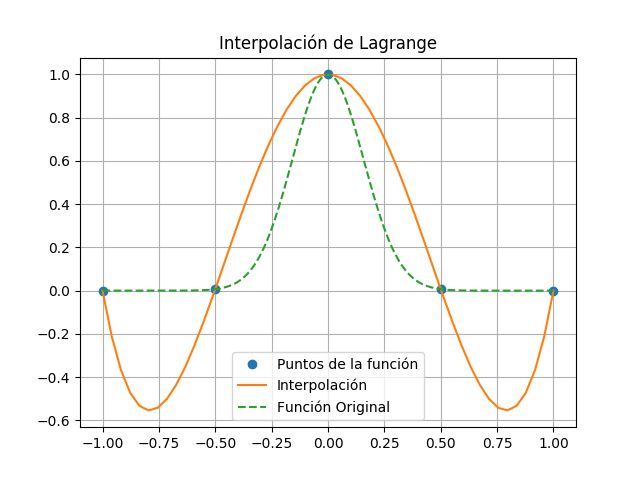
\includegraphics[height=8cm]{P1_1.png}
  \caption{Interpolación polinomial con 5 puntos.}
  \label{P1_1}
\end{figure}


En el siguiente gráfico, figura \ref{P1_2}, vemos como con
distinta cantidad de puntos, nuestra interpolación va mejorando,
pero notamos que la interpolación converge cerca del centro, no
así en los extremos, donde vemos que oscila alejándose demasiado
de la función original. De todas maneras vemos como con 30
puntos estas desviaciones de la función original son muy cerca
de los bordes y no tan pronunciadas ni altas como lo es con 15
puntos.



\begin{figure}[H]
  \centering
  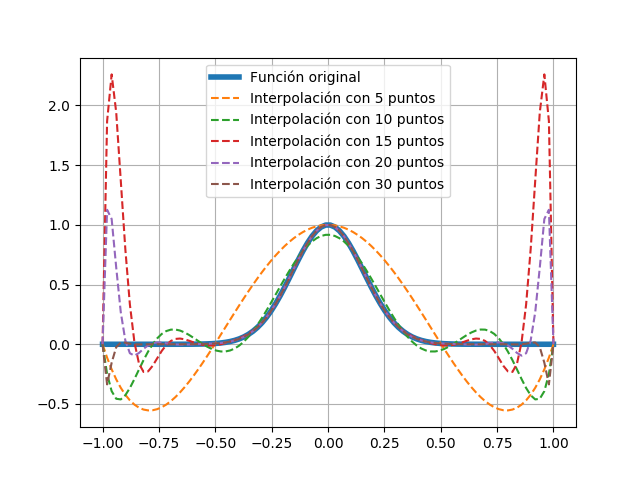
\includegraphics[height=8cm]{P1_2.png}
  \caption{Interpolaciones con polinomios\\ para varios puntos equiespaciados}
  \label{P1_2}
\end{figure}


Es interesante, notar cómo se comportan estas oscilaciones.
Podemos intentar caracterizarlas buscando los valores máximos de
las desviaciones entre las interpolaciones y la función
original. Para esto podemos restar la función original con cada
interpolación, sacar el valor absoluto de esta resta y
finalmente tomar el máximo de este nuevo arreglo, haciendo esto
para distintas cantidades de puntos, obtenemos el gráfico de la
figura \ref{P1_3}. En este gráfico vemos el comportamiento de la
interpolación y notamos que al rededor de n=40 puntos recién
tenemos algo que podríamos aventurarnos a considerar una buena
interpolación, sin siquiera ver el gráfico de la interpolación.


\begin{figure}[H]
  \centering
  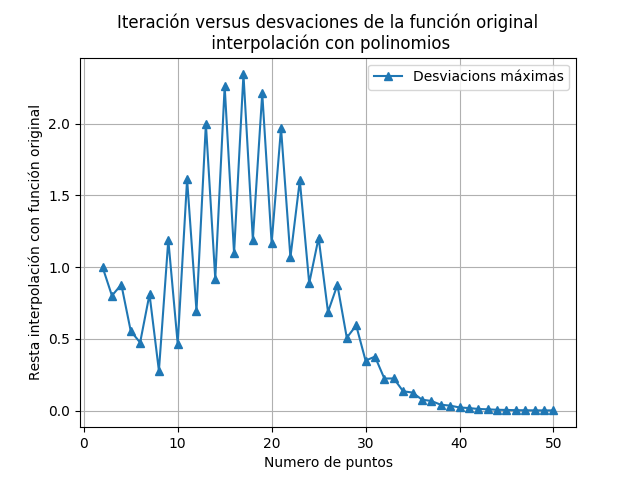
\includegraphics[height=8cm]{P1_3.png}
  \caption{Máximas desviaciones: interpolación polinomial}
  \label{P1_3}
\end{figure}




\subsection{Spline.}

Si bien para Lagrange se implementó el algoritmo desde cero,
para Spline vamos a estar usando scipy, ya que es un poco
más complejo de implementar y tomaría mucho tiempo en eso,
que no es el foco de este informe. Para el spline de scipy vamos
a usar CubicSpline con el parámetro \emph{bc\_type = ``natural''}, lo que quiere decir que nuestra interpolación va a
tener segundas derivadas igual a cero en los extremos, además de
ser continua.

\subsubsection{Sobre la implementación de CubicSpline.}

Si vamos a la \href{https://github.com/scipy/scipy/blob/v1.3.0/scipy/interpolate/_cubic.py#L454-L837}{documentación de scipy
sobre CubicSpline}, podemos notar que la implementación toma en
cuenta todos los casos posibles de funciones que podrían
interesarnos. En el caso general (línea 591) vemos que toma los
valores que se le entrega a la función, para armar un sistema de
ecuación que en forma matricial, busca los valores de la segunda
derivada en cada punto dado. Imponiendo continuidad y que la
primera derivada sea suave, logra encontrar una solución única
para un conjunto de puntos cualquiera. Para resolver el sistema,
usa un solver que tiene también en la librería.


\subsubsection{Spline.}
Veamos los mismos gráficos que vimos para el caso de
interpolación con polinomios.

Para el primer gráfico, figura \ref{P1_S_1}, vemos que hay una
mejora inmediata con respecto a la interpolación anterior, ya
que vemos que el mínimo de la interpolación Spline, es mayor que
el de la interpolación polinomial.

\begin{figure}[H]
  \centering
  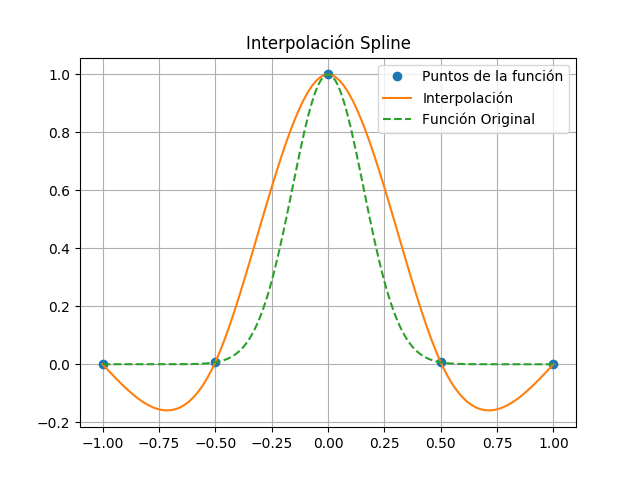
\includegraphics[height=8cm]{P1_S_1.png}
  \caption{Interpolación Spline con 5 puntos.}
  \label{P1_S_1}
\end{figure}



En la figura \ref{P1_S_2} notamos cómo mejora sustancialmente la interpolación a medida que agregamos puntos, de hecho la mejora es tal, que a partir de los 15 puntos, las ganancias en precisión de la interpolación es imperceptible a simple vista.
Esto lo podemos corroborar viendo el gráfico de la figura \ref{P1_S_3}, en donde claramente a partir de los 15 puntos no obtenemos mejoras.







\begin{figure}[H]
  \centering
  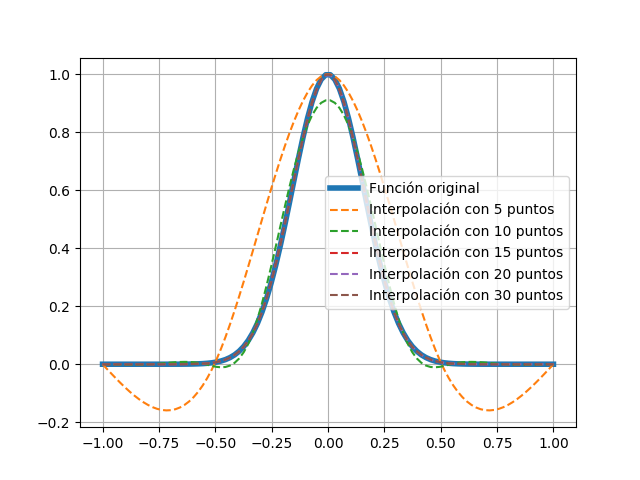
\includegraphics[height=8cm]{P1_S_2.png}
  \caption{Interpolaciones Spline\\ para varios puntos equiespaciados}
  \label{P1_S_2}
\end{figure}


\begin{figure}[H]
  \centering
  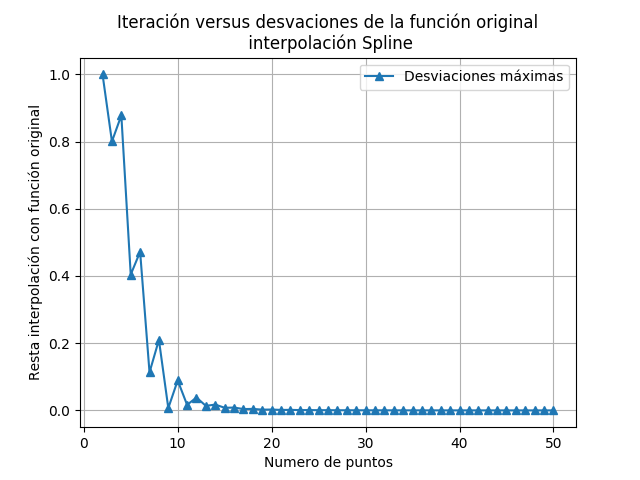
\includegraphics[height=8cm]{P1_S_3.png}
  \caption{Máximas desviaciones: interpolación Spline}
  \label{P1_S_3}
\end{figure}




\newpage

\section{Pregunta 2.}


En la primera parte de esta pregunta se nos pide
interpolar el valor de la anomalía para el año 2016.
Para esto vamos a intentar 3 manera de interpolar los
datos. Las dos primeras, son las más directas, que es
tomar los datos de los promedios y aplicar las
interpolaciones de la parte anterior. La tercera es
tomar los datos de todos los meses que disponemos,
para interpolar los datos de los meses del 2016 y así
obtener un promedios.
En la figura \ref{P2_1} tenemos los datos junto con las distintas interpolaciones, además del valor real medido para el año 2016. Al contrario de como vimos en la primera parte, la interpolación que mejor se ajustó al dato realmente medido fue la polinomial.


\begin{figure}[H]
  \centering
  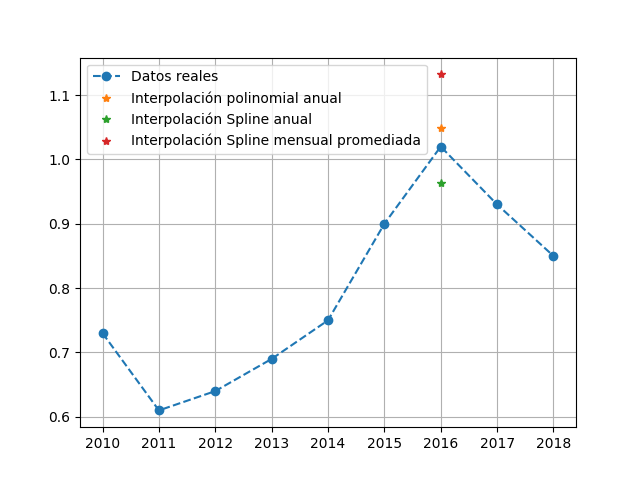
\includegraphics[height=8cm]{P2_1.png}
  \caption{Anomalías interpoladas y medidas.}
  \label{P2_1}
\end{figure}






\newpage

\section{Discusión y Conclusiones}

Para la primera parte de la tarea, vimos como distintas interpolaciones pueden dar resultados muy distintos, y vimos cómo el resultado dependía mucho de la cantidad de puntos entregados.

Para la segunda parte, tenemos que contrario a la primera, la polinomial fue la mejor interpolación para este caso. Las razones pueden ser las siguientes:

En primer lugar, los promedio no caracterizan bien las fluctuaciones reales de los datos, esto es más fácil de ver en la figura \ref{P2_2} donde notamos que el comportamiento de los datos por mes difiere mucho del comportamiento en promedio anual, por lo que no es un buen muestreo el tener un dato al año, para intentar compensar esto, se hizo una interpolación spline en todos los meses, pero acá surgió otro problema, ahora los datos que faltaban son más, y no solo eso, sino que son muchos datos juntos (12, uno por mes) por lo que una interpolación spline no tiene suficiente información para garantizar un buen resultado en el intervalo solicitado. Finalmente, es posible que la interpolación polinomial haya funcionado con un poco de suerte, ya que en otras circunstancias no se habría desempeñado tan bien.


\begin{figure}[H]
  \centering
  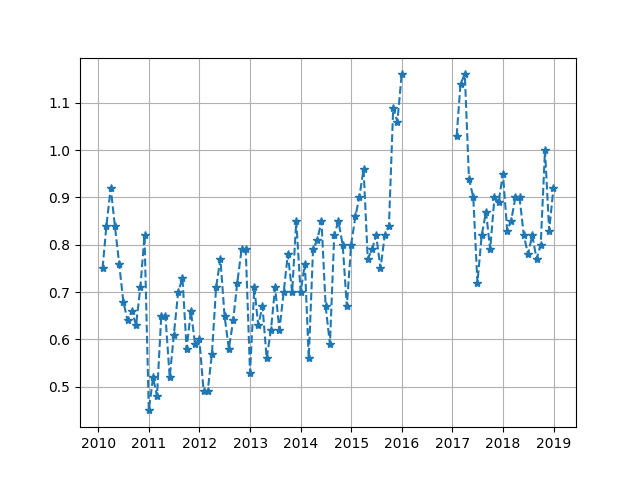
\includegraphics[height=8cm]{P2_2.png}
  \caption{Anomalías por mes.}
  \label{P2_2}
\end{figure}





\end{document}
